%%%%%%%% ICML 2023 EXAMPLE LATEX SUBMISSION FILE %%%%%%%%%%%%%%%%%

\documentclass{article}

% Recommended, but optional, packages for figures and better typesetting:
\usepackage{microtype}
\usepackage{graphicx}
\usepackage{subfigure}
\usepackage{booktabs} % for professional tables

\usepackage{tikz}
% Corporate Design of the University of Tübingen
% Primary Colors
\definecolor{TUred}{RGB}{165,30,55}
\definecolor{TUgold}{RGB}{180,160,105}
\definecolor{TUdark}{RGB}{50,65,75}
\definecolor{TUgray}{RGB}{175,179,183}

% Secondary Colors
\definecolor{TUdarkblue}{RGB}{65,90,140}
\definecolor{TUblue}{RGB}{0,105,170}
\definecolor{TUlightblue}{RGB}{80,170,200}
\definecolor{TUlightgreen}{RGB}{130,185,160}
\definecolor{TUgreen}{RGB}{125,165,75}
\definecolor{TUdarkgreen}{RGB}{50,110,30}
\definecolor{TUocre}{RGB}{200,80,60}
\definecolor{TUviolet}{RGB}{175,110,150}
\definecolor{TUmauve}{RGB}{180,160,150}
\definecolor{TUbeige}{RGB}{215,180,105}
\definecolor{TUorange}{RGB}{210,150,0}
\definecolor{TUbrown}{RGB}{145,105,70}

% hyperref makes hyperlinks in the resulting PDF.
% If your build breaks (sometimes temporarily if a hyperlink spans a page)
% please comment out the following usepackage line and replace
% \usepackage{icml2023} with \usepackage[nohyperref]{icml2023} above.
\usepackage{hyperref}


% Attempt to make hyperref and algorithmic work together better:
\newcommand{\theHalgorithm}{\arabic{algorithm}}

\usepackage[accepted]{icml2023}

% For theorems and such
\usepackage{amsmath}
\usepackage{amssymb}
\usepackage{mathtools}
\usepackage{amsthm}

% if you use cleveref..
\usepackage[capitalize,noabbrev]{cleveref}

%%%%%%%%%%%%%%%%%%%%%%%%%%%%%%%%
% THEOREMS
%%%%%%%%%%%%%%%%%%%%%%%%%%%%%%%%
\theoremstyle{plain}
\newtheorem{theorem}{Theorem}[section]
\newtheorem{proposition}[theorem]{Proposition}
\newtheorem{lemma}[theorem]{Lemma}
\newtheorem{corollary}[theorem]{Corollary}
\theoremstyle{definition}
\newtheorem{definition}[theorem]{Definition}
\newtheorem{assumption}[theorem]{Assumption}
\theoremstyle{remark}
\newtheorem{remark}[theorem]{Remark}

% Todonotes is useful during development; simply uncomment the next line
%    and comment out the line below the next line to turn off comments
%\usepackage[disable,textsize=tiny]{todonotes}
\usepackage[textsize=tiny]{todonotes}
\usepackage{comment}

% The \icmltitle you define below is probably too long as a header.
% Therefore, a short form for the running title is supplied here:
\icmltitlerunning{H2Ope - Is there any for our fresh water?}

\begin{comment}
Title Suggestions

- Fresh water - is it really that fresh
- Fresh water - How little is little?
- FRESH: Free (Water) Resource Estimates Shrink Harshly
- H2Ope - Is there any for our fresh water?
- DROWN - Daily Rain Owes Water Nothing
- CHRIS - CHRIStian
- 404 - Fresh Water not found
- 403 - Not authorized to access fresh water
- 402 - Payment required for fresh water

- WATERWISE - Worldwide Analysis of Treatment, Exploitation, Resources, and WIse Sourcing Evaluation
- AQUASTAT - Analysis of QUAlity, Sourcing, Treatment, Accessibility, and Trends in Global Water Use
- H2OPE - Is there any for our fresh water?
- H2OPE - H2O (Water) Policy and Economics: A Statistical Evaluation of International Water Management
- STREAM - Statistical Trends in Resources, Exploitation, Access, and Management of Water Globally
- GLOBEWET - GLObal Benchmarking and Evaluation of Water Efficiency and Treatment
\end{comment}


\begin{document}
\twocolumn[
\icmltitle{Assessing the Blue Planet: Global Insights on Freshwater Challenges and Management Strategies}
%\icmltitle{The Blue Planet Under Pressure: TODO}
%\icmltitle{Assessing the Blue Planet: Why money matters in the fight against water scarcity}

% It is OKAY to include author information, even for blind
% submissions: the style file will automatically remove it for you
% unless you've provided the [accepted] option to the icml2023
% package.

% List of affiliations: The first argument should be a (short)
% identifier you will use later to specify author affiliations
% Academic affiliations should list Department, University, City, Region, Country
% Industry affiliations should list Company, City, Region, Country

% You can specify symbols, otherwise they are numbered in order.
% Ideally, you should not use this facility. Affiliations will be numbered
% in order of appearance and this is the preferred way.
\icmlsetsymbol{equal}{*}

\begin{icmlauthorlist}
\icmlauthor{Simon Fehrenbach}{equal,first}
\icmlauthor{Christian Jestädt}{equal,second}
\icmlauthor{Marten Kreis}{equal,third}
\icmlauthor{Josef Müller}{equal,fourth}
\end{icmlauthorlist}

% fill in your matrikelnummer, email address, degree, for each group member
\icmlaffiliation{first}{5451553, simon.fehrenbach@gmail.com, Bsc Sociology with a minor in Computer Science}
\icmlaffiliation{second}{6071013, christian.jestaedt@student.uni-tuebingen.de, BSc Informatik}
\icmlaffiliation{third}{6570772, marten.kreis@student.uni-tuebingen.de, MSc Computer Informatics}
\icmlaffiliation{fourth}{6565774, josef.mueller@student.uni-tuebingen.de, MSc Computer Informatics}

% You may provide any keywords that you
% find helpful for describing your paper; these are used to populate
% the "keywords" metadata in the PDF but will not be shown in the document
\icmlkeywords{AQUASTAT, ICML}

\vskip 0.3in
]

% this must go after the closing bracket ] following \twocolumn[ ...

% This command actually creates the footnote in the first column
% listing the affiliations and the copyright notice.
% The command takes one argument, which is text to display at the start of the footnote.
% The \icmlEqualContribution command is standard text for equal contribution.
% Remove it (just {}) if you do not need this facility.

%\printAffiliationsAndNotice{}  % leave blank if no need to mention equal contribution
\printAffiliationsAndNotice{\icmlEqualContribution} % otherwise use the standard text.

\begin{abstract}
Globally, around 4 trillion cubic meters of water are consumed every year. However, 97.5\% of the total water resources available on this planet consist of salt water. Thus, the access to a freshwater supply is of critical importance. 

In this work, we use global data to analyze and illustrate the availability, usage, and treatment of freshwater on a worldwide scale. Two significant factors influencing water stress levels have been identified: population growth and changes in precipitation patterns. Additionally, it is noted that various strategies are employed to cope with water scarcity. Countries experiencing high water stress levels tend to allocate a greater proportion of available water resources to the agricultural sector. However, the treatment of wastewater appears to be primarily influenced by different factors. 
\begin{comment}
The primary source of data for this project is the \href{https://data.apps.fao.org/aquastat/?lang=en}{FAO AQUASTAT} dataset, which encompasses a broad range of metrics over time regarding freshwater withdrawal in different sectors, pressure on the freshwater resources and irrigation and drainage. Different visualization methods and statistical tests are employed to understand the causes and consequences of water scarcity.
\end{comment}
\end{abstract}

\begin{comment}
Put your abstract here. Mention, in two sentences, what you are planning to work on. 
Then, mention which dataset you are planning to use. Include \href{https://noaadata.apps.nsidc.org/NOAA/G02135/south/daily/data/}{a link} to the dataset you are planning to use (If you are planning to collect your own data, explain how you are going to do so). If possible, mention (one sentendependce) how you came across this dataset, or why you decided to do this. Explain what kind of analysis you are planning. Finally, declare which results your are expecting to achieve. Your entire abstract should be at most 20 lines long.
\end{comment}

\begin{comment}
1: Beginning:
    - Bestimmung der Dimension werden zusammen diskutierts
2: Aufteilung der verschiedenen Untersuchungsaspekte auf die Projektteilnehmer
    - eventuelle Gemeinsamkeiten zwischen den Aspekten führen zur Zusammenarbeit
    - eventuell gibt es einzelne Aspekte, die alleine analysiert werden
\end{comment}

% https://simon.peytonjones.org/great-research-paper/
\begin{comment}
4. Introduction
    - Datensatz vorstellen
    - Fragen von Ergebnissen ableiten auch mit Hinblick, dass da eine tiefere Analyse möglich sein könnte
1. Methods:
    - "Was hast du gemacht (ohne Ergebnisse zu erwähnen)?"
    - Datensätze
    - Analysemethoden
    - Preprocessing
    - Tests
    - Vorgehen bei Formeln
    - evtl. Reflexion bei den Methoden -> "als erstes hab ich Plan A gemacht, aber das hat nicht geklappt, deswegen Plan B"
2. Results
    - 
3. Discussion
\end{comment}

\section{Introduction}
In today's world, the importance of freshwater cannot be overstated. It is not only essential for basic human needs like drinking and agriculture, but also for industrial activities. However, with the growing global population and environmental changes, freshwater is becoming increasingly scarce in many regions. This situation has led to increased \textit{water stress}, defined as the ratio of freshwater withdrawal to its availability. Alarmingly, this ratio has exceeded 100\% in some countries, indicating that more water is used than is naturally available. % TODO: water stress defined twice => can be removed?

This project aims to provide a comprehensive review of the predominant factors influencing global water withdrawal by investigating the impact of population growth and potential consequences of climate change. It explores the underlying causes of water stress and examines different water management strategies adopted by countries that are impacted by water scarcity. This report also illustrates the significant role that financial resources play in the access to clean water. Special attention is paid to agricultural water usage, which significantly contributes to the escalating demand for water. However, it's important to note that the scope of this paper is to provide a preliminary overview.\\
%setting the stage for more comprehensive analyses in the future.\\ safe nicht?

\section{Methods}

% Introduction
The \textit{AQUASTAT} dataset \cite{FAO2021}, developed by the \textit{Food and Agriculture Organization of the United Nations}, is the primary resource used in this analysis. It features an extensive compilation of over 193 different variables and indicators, gathered across 200 countries over a span of up to 57 years. The dataset encompasses information on water resources and their utilization, including water withdrawal, wastewater, pressure on water resources, as well as aspects related to irrigation, drainage, environment, and health.

% Water Stress
Analyzing the \textit{water stress} indicator lets us identify the countries which are facing water scarcity issues, and helps us focus our data analysis on the areas that are mostly impacted.
% Definition
% TODO: Gibt scheinbar auch noch andere Faktoren die das beeinflussen, auch wenn die korrelation relativ hoch ist. Siehe: https://yaon.org/scarcity_stress.png
Water stress is defined as the freshwater withdrawal as a proportion of available freshwater resources \cite{UN_SDG642}. Countries that have an increased demand for fresh water or a decline in fresh water resource availability face higher water stress.\\
\begin{comment}
It can be computed as follows:
\begin{align}
    y_{\text{stress}} = 100 \cdot \frac{x_{\text{tfw}}}{x_{\text{trwr}} - x_{\text{efr}}}
\end{align}
where $y_{\text{stress}}$ is the water stress, $x_{\text{tfw}}$ the total freshwater withdrawal, $x_{\text{trwr}}$ the total renewable water resources and $x_{\text{efr}}$ the environmental flow requirements. 
\end{comment}
% ================ Factors that contribute to water stress ================
To identify the factors that have the highest impact on the water stress variable of a country, different statistical tests are conducted.\\\\
% ================ TEST: Population ================
Initially, we examine the influence of the population on a countries total water withdrawal, given the presumption of a substantial interconnection between the two. To test this, we plot the variables over time and compute their correlation. Furthermore, we construct a hypothesis test where countries are divided into two groups based on their respective population size. The \textit{total water withdrawal} variable is repeatedly rearranged, generating a total of $n = 100.000$ permutations. To compare the obtained results for both groups, the following metric is applied:
\begin{align}
    T = \left[\frac{1}{n}\cdot\sum_{i \in G_1} X_i\right] - \left[\frac{1}{n}\cdot\sum_{i \in G_2} Y_i\right]
\end{align}
where $X_i$ and $Y_i$ are permuted the total water withdrawal samples of their respective groups $G_1$ and $G_2$. After obtaining the distribution for $n$ samples under the null hypothesis, we determine the $p$-value by comparing our result to the actual value of the dataset, which was calculated using the same metric.\\
% ================ Climate change ================
The second factor we investigate is climate change. Previous work shows that different global climate models estimate a future increase in water stress impacting between 0.5 and 3.1 billion people by the year 2050 \cite{Gosling2016, Stringer2021}. To identify countries currently affected by climate-induced water stress, geospatial data for temperature anomalies \cite{Temp_NOAA2022} and mean precipitation levels \cite{Precip_NOAA2022} are visualized, as they are among the most significant contributing factors to freshwater availability \cite{Berghuijs2017}. The datasets are provided by the \textit{National Oceanic and Atmospheric Administration} (NOAA). 
\begin{comment}
Furthermore, we compare time series data for global temperature \cite{TempTS_NOAA2023} and precipitation anomalies \cite{Blunden2020} from 1900 to 2021. We employ linear regression to model the data, with the year serving as the input variable and the predicted output being the anomaly. This analysis aims to determine whether a similar trend, analogous to the global temperature increase, is observed in precipitation patterns.
\end{comment}
\\\\
% ================ Water Management strategies ================
% den part hab ich rausgenommen, weil wir den platz dafür nicht mehr haben. Können die paar vergleiche mit der schon existierenden water stress map machen 
%- test if countries that have higher stress tend to irrigate their crops with treated water
Shifting the focus to a related concern, we investigate how countries that suffer from high water stress spend their available water resources. The water consumption is distinguished between three different sectors, the agricultural, industrial and municipal sector.
% water scarcity korrelliert sogar ganz leicht negativ mit Unterernährung (-0.1), da reiche Länder eher water scarcity besitzen
To provide a stable and sufficient food supply for the population of a country, the agricultural water withdrawal is essential. We want to examine whether countries that have high water stress levels spend a larger share of their available water on the agricultural sector. To explore this hypothesis, a \textit{Kruskal Wallis} test is performed. The countries are distributed in three groups, with the water stress level being the sorting criterion. The \textit{Kruskal Wallis} test statistic $H$ is approximately \textit{chi-squared} distributed and can be computed as follows:
\begin{align}
    H = \left(\frac{12}{N(N+1)} \sum_{j = 1}^k \frac{R_j^2}{n_j}\right) -3(N+1)
\end{align}
where $N$ is the total number of samples, $n_j$ the sample size for group $j$ and $R_j$ the sum of ranks of the $j$-th group \cite{Ostertagova2014}.
Before conducting the test, the data undergoes visual analysis using $PP$ and $QQ$-plots to ascertain its adherence to the test prerequisites.\\\\
% - looking at managment strategies by plotting wastewater treatment
Building upon the analysis of water stress and resource allocation, the investigation of water management strategies also extends to an examination of wastewater management practices. The \textit{WateReuse Association} defines wastewater as “the used water of a community or industry that contains dissolved and suspended matter”.
This study plots the ratio of \textit{treated} wastewater to \textit{total} wastewater per country in 2012, creating a baseline. We then visualize the progression in wastewater treatment up to 2020 by plotting the relative growth of this ratio. The relative growth measures the change in wastewater management as a proportion to the data in 2012. This metric is useful for evaluating the development of wastewater strategies in response to water stress and identifying regional variations.
% ================ Drinking water & water availability ================

After reviewing water management practices, it logically follows to explore the differences in making water resources usable, particularly in meeting the needs of the population.
As currently over one billion people do not have access to safe drinking water \cite{Programme2023}, it is crucial to determine if this issue predominantly affects countries experiencing high water stress.
Scatterplots allow for better visual identification of trends and general distribution patterns, providing a clear overview of these issues.
In this approach, the relationships between water stress, GDP per capita, and access to clean drinking water are plotted to identify interesting influences through visual analysis. 
Due to an enormous water stress in a few countries, the variable was capped at 175\%.

\section{Results}
\label{sec:results}
% ============== Population test ================
The conducted analysis indicates a strong correlation ($r = 0.93$) between \textit{total freshwater withdrawal} and \textit{population}, highlighting a significant relationship between these two variables. With a steady increase in population, there is a parallel rise in freshwater demand, intensifying the strain on existing water resources. It is noteworthy that the majority of water consumption is attributed to agricultural activities, which play a crucial role in sustaining the population through food production.
\begin{comment}
\begin{figure}[!ht]
    \centering
    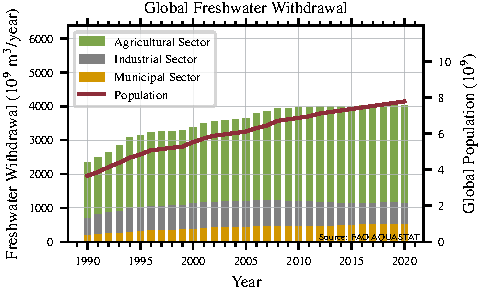
\includegraphics{fig/global_water_withdrawal.pdf}
    \caption{Comparing the global freshwater withdrawal to the global population from 1990 to 2020, the water usage is categorized into three different sectors.}
    \label{fig:test:population1}
\end{figure}
\end{comment}
The conducted hypothesis test through permutation with the null hypothesis $H_0$ stating that the variable \textit{population} has no effect on the \textit{total water withdrawal} can be rejected, since we obtain a $p$-value smaller than $1\cdot10^{-5}$.

% ============== Climate Change ================
\begin{figure}[!ht]
    \centering
    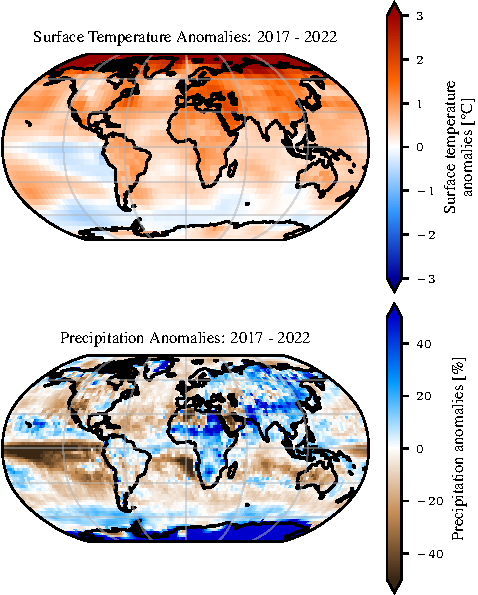
\includegraphics{fig/temp_precip_spatial.pdf}
    \caption{Surface temperature (1971 to 2000 baseline) and precipitation anomalies (1979 to 2000 baseline) for a time interval of six years from 2017-2022. While all countries are directly impacted by increasing surface temperatures, a decrease in precipitation only affects certain regions.}
    \label{fig:climate1}
\end{figure}
The analysis of the influence of climate change on water stress using geospatial data, shown in \autoref{fig:climate1}, indicates that rising surface temperatures affect all countries, leading to heightened evaporation. Conversely, we also observe that decreases in precipitation seem to be concentrated in specific regions. This shift in precipitation patterns results in heightened rainfall in other areas. Since precipitation is an important factor influencing renewable freshwater availability, especially surface water and groundwater, this can drastically change the water stress level of affected countries. Areas that are mostly impacted by reduced precipitation of up to 50\% as North Africa, the Arabian Peninsula, Australia, and North America.

Next, the current water stress levels are visualized to identify countries that currently suffer from water scarcity. 
\begin{figure}
    \centering
    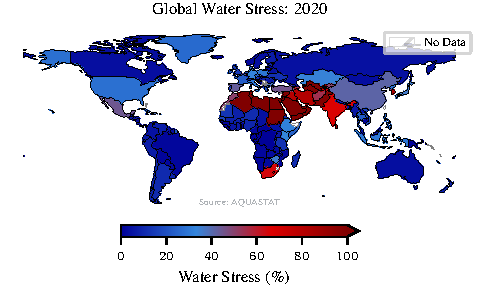
\includegraphics{fig/global_water_stress.pdf}
    \caption{2020 Global Water Stress Levels: The vast difference of global water stress levels can be perceived when comparing North- and South Africa and South-eastern countries to the rest of the world.}
    \label{fig:water_stress1}
\end{figure}
As illustrated in \autoref{fig:water_stress1} one can observe that some countries with high water stress levels are also heavily impacted by reduced precipitation. Since this metric implies that a large amount of the renewable freshwater resources are already consumed by the respective countries, various measures and strategies must be adopted \cite{Tortajada2019, Belhassan2021} to counteract this.

The initial strategy investigated is whether countries facing high water stress allocate a larger proportion of their freshwater withdrawals to agriculture, a sector critical for food supply and a major consumer of water resources. The conducted analysis shows that countries that face high water stress levels use a far larger share of the available water for agricultural purposes. For nations with water stress levels over 40\% the median share of water allocated for the agricultural sector is 75\% while for countries with water stress levels under 20\% the median share reduces to 51\%. The $p$-value for the performed \textit{Kruskal Wallis} test with the null hypothesis $H_0$ stating all mean group ranks are equal independent of their respective stress levels is 0.01.

% ============== Wastewater Management ================
Another aspect we explore is wastewater management, encompassing water treatment and reuse.  
\begin{figure}[!ht]
    \centering
    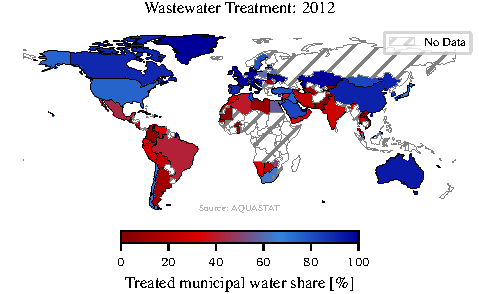
\includegraphics{fig/fig_world_map_Treated_municipal_water_share_2012.pdf}
    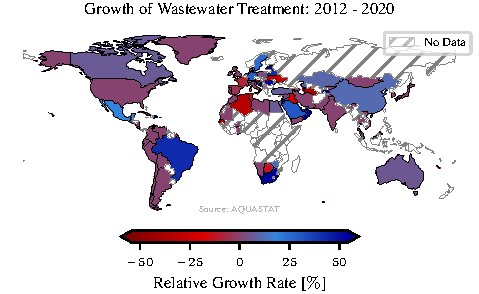
\includegraphics{fig/fig_growth_rate_Treated_municipal_water_share.pdf}
    \caption{Change in Proportion of Treated Municipal Wastewater to Total Wastewater (2012 to 2020 baseline): Countries that face high water stress (\autoref{fig:water_stress1}) show minimal to no alterations in treatment practices.}
    \label{fig:change_treated_wastewater_share}
\end{figure}
\autoref{fig:change_treated_wastewater_share} highlights a significant divide in wastewater treatment across the globe.
Developed countries generally tend to treat a large portion of their wastewater, in stark contrast to many countries in the global south. Regions experiencing high water stress seem to have lower rates of municipal wastewater treatment, though some countries on the Arabian Peninsula (Saudi Arabia, UAE) are an exception with higher treatment levels than other countries in their region. Furthermore, when this data is compared to areas most impacted by negative rainfall anomalies and even by water stress, similar disparities in the increase in water treatment are observed. 

% ============== Drinking water ================
% !! Hier würde ich die achsen umdrehen, weil gerade GDP und Water Stress die abhängigen variablen sind
% => klingt gut, ich mach auch gerade mal die achsenbeschriftungen
\begin{figure}[!ht]
    \centering
    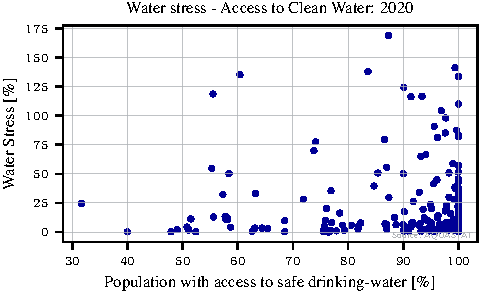
\includegraphics{fig/fig_Water stress - access to clean water: 2020.pdf}
    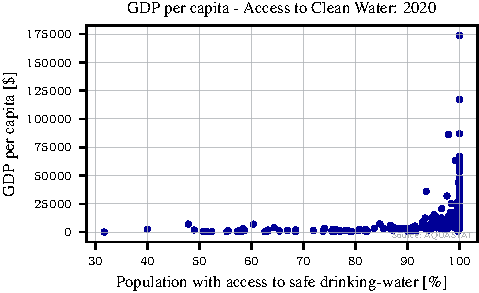
\includegraphics{fig/fig_GDP per capita - access to clean water: 2020.pdf}
    \caption{Correlations between \textit{total population with access to safe drinking water} and \textit{GDP per capita} and \textit{water stress levels} respectively}
    \label{fig:water_stress_access}
    \label{fig:gdp_access}
\end{figure}
Examining the relationship between access to safe drinking water and water stress in 2020 (\autoref{fig:water_stress_access}) reveals no straightforward link. Countries exhibit varying levels of water stress yet can have both high and low access to safe drinking water, indicating that factors apart from water stress alone may play significant roles in determining water accessibility.\\
When considering GDP per capita in relation to access to safe drinking water (\autoref{fig:gdp_access}), a much stronger association is evident. All countries with limited access to safe drinking water also exhibit a lower GDP per capita, suggesting that economic strength is a crucial factor in ensuring the availability of safe drinking water.

%TODO: hier brauchen wir bitte noch Einheiten an den achsen, also bei gdp [$] und bei total population den faktor, mit dem multipliziert wurde (10^6, eventuell)? pffffff, wer braucht den sowas

% ideas to connect this paragraph with the rest of the paper: rainfall, unterernährung, landwirtschaft
% done: scarcity, gdp
%hihi
% existing: unterernährung, rainfall


\section{Discussion}
In \autoref{sec:results}, we identified population growth and climate change as the predominant factors of high water stress. As the population growths, more food has to be produced, which is increases the demand of water in the agricultural sector. This is also underlined by our finding that countries with high water stress often prioritize water allocation for the agricultural sector. The impact of climate change, on the other hand, is much more difficult to quantify. Our analysis shows that shifting precipitation patterns affect specific regions, potentially leading to water scarcity and impacting food supply. The precipitation dataset helped identify affected countries, laying the groundwork for future predictive models on precipitation trends.

The examination of wastewater treatment reveals that economic factors and developmental progress seem to exert a significantly greater impact on advancements in water treatment technologies than the immediate need for water reclamation, which arises from high water stress and limited precipitation. But although it appears intuitive that development and therefore economic factors coincide with enhanced water treatment capabilities, further analysis is necessary to fully understand the underlying reasons for the observed discrepancies.\\
Similar dynamics seem to be at play regarding access to clean drinking water. Water stress does not appear to be a major determinant of this access, hinting that scarce water resources may not be the main determinant of this issue. Instead, a clear link can be observed with GDP per capita, as no country with restricted access to clean drinking water has a GDP akin to those countries in the “developed world”. This devalues water stress as an indicator, giving poor countries their whole own set of problems and opening up more topics for subsequent research.\\
Furthermore, this overview of water access and treatment strategies, though preliminary and in need of further investigation, highlights how discussions on technical solutions for the impacts of climate change need to include the significant role of financial resources. Many countries appear to already face challenges in making water accessible to their populations, hindering their ability to consider more advanced, technologically intensive, and costly water management strategies.

\section*{Contribution Statement}

Simon Fehrenbach performed a comprehensive analysis of global wastewater treatment strategies, assessing their effectiveness and sustainability.
Christian Jestädt explored the factors influencing water stress and availability, including environmental and human-driven elements.
Marten Kreis executed the statistical analysis, correlating precipitation, temperature, and population data.
Josef Müller assisted in researching wastewater strategies and maintained the \href{https://github.com/am9zZWY/team-aqua}{codebase} for data analysis and visualization.
All authors contributed equally to the development of visualizations and the writing of the report.


% klingt bisschen nach fleischwolf. Aber können auch gerne gleich mal gemeinsam drüber?

% ================ Unseres ===========
%As shown in \autoref{sec:results}, the two predominant factors responsible for high water stress are population growth and climate change. The main reason for a connection between water withdrawal and population might be the necessity to provide more food and thus increasing the agricultural water withdrawal. This is also underlined by the analysis, which indicated that countries with high water stress prioritize water allocation towards the agricultural sector.\\
%The impact of climate change, on the other hand, is much more difficult to quantify. Our analysis revealed that precipitation patterns are shifted, impacting specific regions. This can lead to severe water scarcity issues and droughts, which might compromise the food supply. Countries which are increasingly impacted by this need to explore various measures to counteract the issues that arise due to climate change. The precipitation dataset was used to obtain an overview of the current precipitation anomalies and to identify impacted countries. Subsequent research could build upon this foundation and construct prediction models, such as regression models, to forecast future precipitation levels.
%\\\\
%The examination of wastewater treatment reveals that economic factors and developmental progress seem to exert a significantly greater impact on advancements in water treatment technologies than the immediate need for water reclamation, which arises from high water stress and limited precipitation. But although it appears intuitive that development and therefore economic factors coincide with enhanced water treatment capabilities, further analysis is necessary to fully understand the underlying reasons for the observed discrepancies.\\
%Similar dynamics seem to be at play regarding access to clean drinking water. Water stress does not appear to be a major determinant of this access, hinting that scarce water resources may not be the main determinant for this issue. Instead, a clear link can be observed with GDP per capita, as no country with restricted access to clean drinking water has a GDP akin to those countries in the "developed world." This devalues water stress as an indicator, giving poor countries their whole own set of problems and opening up more topics for subsequent research.\\
%Furthermore, this overview of water access and treatment strategies, though preliminary and in need of further investigation, highlights how discussions on technical solutions for the impacts of climate change need to include the significant role of financial resources. Many countries appear to already face challenges in making water accessible to their populations, hindering their ability to consider more advanced, technologically intensive, and costly water management strategies.



%An issue we encountered is the limitation of the water stress indicator. The indicator normalizes the actual withdrawn renewable freshwater with the potential available renewable freshwater. However, this approach leads to an omission of countries experiencing water scarcity, particularly those with a low GDP per capita.

\bibliography{references.bib}
\bibliographystyle{icml2023}

\end{document}


\begin{comment}
% Outdated:
Christian Jestädt focuses on the graphical visualization of data on map. Simon Fehrenbach prepares the data for visualisation and analysis. Marten Kreis analyses and visualizes water withdrawal over time. Josef Müller focuses on analysing and visualising water treatment and wastewater statistics. All authors will jointly write the text of the report and distribute additional minor visualisation and analysis equally.
\end{comment}
\begin{comment}
- In- and outflow of water
    - analyze:
        - Trinkwasseraufbereitung
        - Regenfall
        - Grundwasser
        - ...
- fresh water withdrawal (normalized) as % of total renewable water resources (wasserknappheit)
    - important quantities: population, water inflow, maybe rain etc.
- 

\end{comment}
\begin{comment}
    (This might also fit into the discussion part)
    - high water scarcity or stress don't seem to be a good indicator for water related problems like access to clean drinking water and undernourishment:
    
    - we see, that the issue of water scarcity is way more complex than reducing it to the effect of a single variable/process (like agriculture)
    - For every variable, there are always a few outliers which have to be looked at seperately (or not at all?)

    - water scarcity depends on the climate and the amount of water used, but the access to clean drinking water depends on a whole different set of variables: water treatment, distribution, and purification. (So mostly costly things)
    (See exp_scatterplot)
    => here we can perfectly talk about the water management strategies

    - doc/water/fig is now synchronised every few minutes with https://team-aqua.yaon.org (upload => from url => select url of image). Let's see if this holds any advantage
\end{comment}



% This document was modified from the file originally made available by
% Pat Langley and Andrea Danyluk for ICML-2K. This version was created
% by Iain Murray in 2018, and modified by Alexandre Bouchard in
% 2019 and 2021 and by Csaba Szepesvari, Gang Niu and Sivan Sabato in 2022.
% Modified again in 2023 by Sivan Sabato and Jonathan Scarlett.
% Previous contributors include Dan Roy, Lise Getoor and Tobias
% Scheffer, which was slightly modified from the 2010 version by
% Thorsten Joachims & Johannes Fuernkranz, slightly modified from the
% 2009 version by Kiri Wagstaff and Sam Roweis's 2008 version, which is
% slightly modified from Prasad Tadepalli's 2007 version which is a
% lightly changed version of the previous year's version by Andrew
% Moore, which was in turn edited from those of Kristian Kersting and
% Codrina Lauth. Alex Smola contributed to the algorithmic style files.
